\documentclass{article}
\author{Zuzanna Dybcio}
\date{October 2023}
\usepackage[utf8]{inputenc}
\usepackage[polish]{babel}
\usepackage[T1]{fontenc}
\usepackage{amsmath}
\usepackage{url}
\usepackage{graphicx}

\begin{document}
Dowiedziałam się dziś (10.10.2023) na spotkaniu DataTeam, że jest możliwość uzyskania dostępu do DataCamp, więc jeśli Pan to czyta, to fajnie by było tę sprawę załatwić ;)
\\\\
\begin{equation}
    N(\overrightarrow{x} | \overrightarrow{\mu}, \Sigma) = \frac{1}{\sqrt{(2\pi)^{D}}} \frac{1}{|\Sigma|} e^{-\frac{(\overrightarrow{x}-\overrightarrow{\mu})^T (\overrightarrow{x}-\overrightarrow{\mu})}{2\Sigma}}
\end{equation}
\\
\begin{equation}
    \text{ln} \space p \space (\overrightarrow{X} | \pi, \mu, \Sigma) \space = \sum_{n=1}^{N} \space \text{ln} \space (\sum_{k=1}^{K} \mathrm \pi_k N \space (\overrightarrow{x_n} | \overrightarrow{\mu_k},\Sigma_k))
\end{equation}
\\
\begin{equation}
    DB = \frac{1}{k} \sum_{i=1}^{k} \space \max_{i \neq j} \space \frac{s_{i} + s_{j}}{d_{ij}}, \space i=1,...,k
\end{equation}
\\\\
Od studiów na kierunku \textbf{\emph{geoinformatyka}} oczekuję zdobycia wiedzy na temat \emph{tworzenia aplikacji geoinformatycznych} i innych powiązanych tematów, ponieważ mam pewne pomysły na zaawansowane projekty z wykorzystaniem \underline{danych przestrzennych}, które by były przydatne dla ludzi (podobne aplikacje jeszcze nie istnieją, a bynajmniej takowych nie odnalazłam), a ja bym mogła na nich \emph{zarobić}. 
\\\\
(Początkowo miałam plan studiować \emph{informatykę} od przyszłego roku (pisałam w tym roku rozszerzenia z matematyki i geografii, lecz by nie stracić roku edukacji, chciałam zacząć teraz jakiekolwiek studia po maturze z geografii i w przyszłym roku przystąpić do rozszerzeń z fizyki oraz informatyki, a że się dowiedziałam, że istnieje coś takiego jak \emph{geoinformatyka}, to tak oto się tu zjawiłam), lecz po dłuższych przemyśleniach doszłam do wniosku, że informatyka jest dziedziną obecnie bardzo popularną. \textbf{Wystarczy odrobina motywacji, by wszystkiego, co na studiach informatycznych jest, nauczyć się samemu} z pomocą np. internetu, co by było trudniejsze w przypadku chęci poszerzenia wiedzy z zakresu geoinformatyki. Uznałam też, że jest to dziedzina bliższa moim zainteresowaniom - \underline{pasjonuje mnie świat, wszechświat i wszelkie nauki ścisłe}, nie tylko konkretne specjalizacje. \emph{Geoinformatyka} jest interdyscyplinarna i to mi się właśnie podoba. Jest jej bliżej do również interesującego mnie \emph{sektora kosmicznego} i \emph{astrofizyki}, niż zwykłej \emph{informatyce}, a także pokrywa się też z moimi pomysłami na projekty.)
\\\\
Od studiów na \textbf{\emph{AGH}} oczekuję możliwości \textbf{poszerzania horyzontów, zdobywania wiedzy}, nie tylko w zakresie jednej specjalizacji, oraz \textbf{rozwijania swoich sportowych pasji}, dlatego chętnie korzystam z oferty przedmiotów innowacyjnych, kół naukowych i AZS.\\\\\\
\textbf{Ulubione seriale:}
\begin{itemize}
    \item The 100
    \item Wyjaśniamy tajemnice umysłu
    \item Wyjaśniamy
    \item Czarne lustro
    \item Stranger Things
\end{itemize}
\textbf{Ulubione piosenki:}
\begin{enumerate}
    \item Avicii - The Nights
    \item Bring Me the Horizon - Throne
    \item Dżem - Wehikuł czasu
    \item Scorpions - Wind of change
    \item Rascall Flatts - Life is a Highway
\end{enumerate}
~\\
\url{https://www.nationalgeographic.com} - treści ciekawe\\
\url{https://stackoverflow.com/} - treści użyteczne ;)
~\\
\begin{figure}[h]
    \centering 
    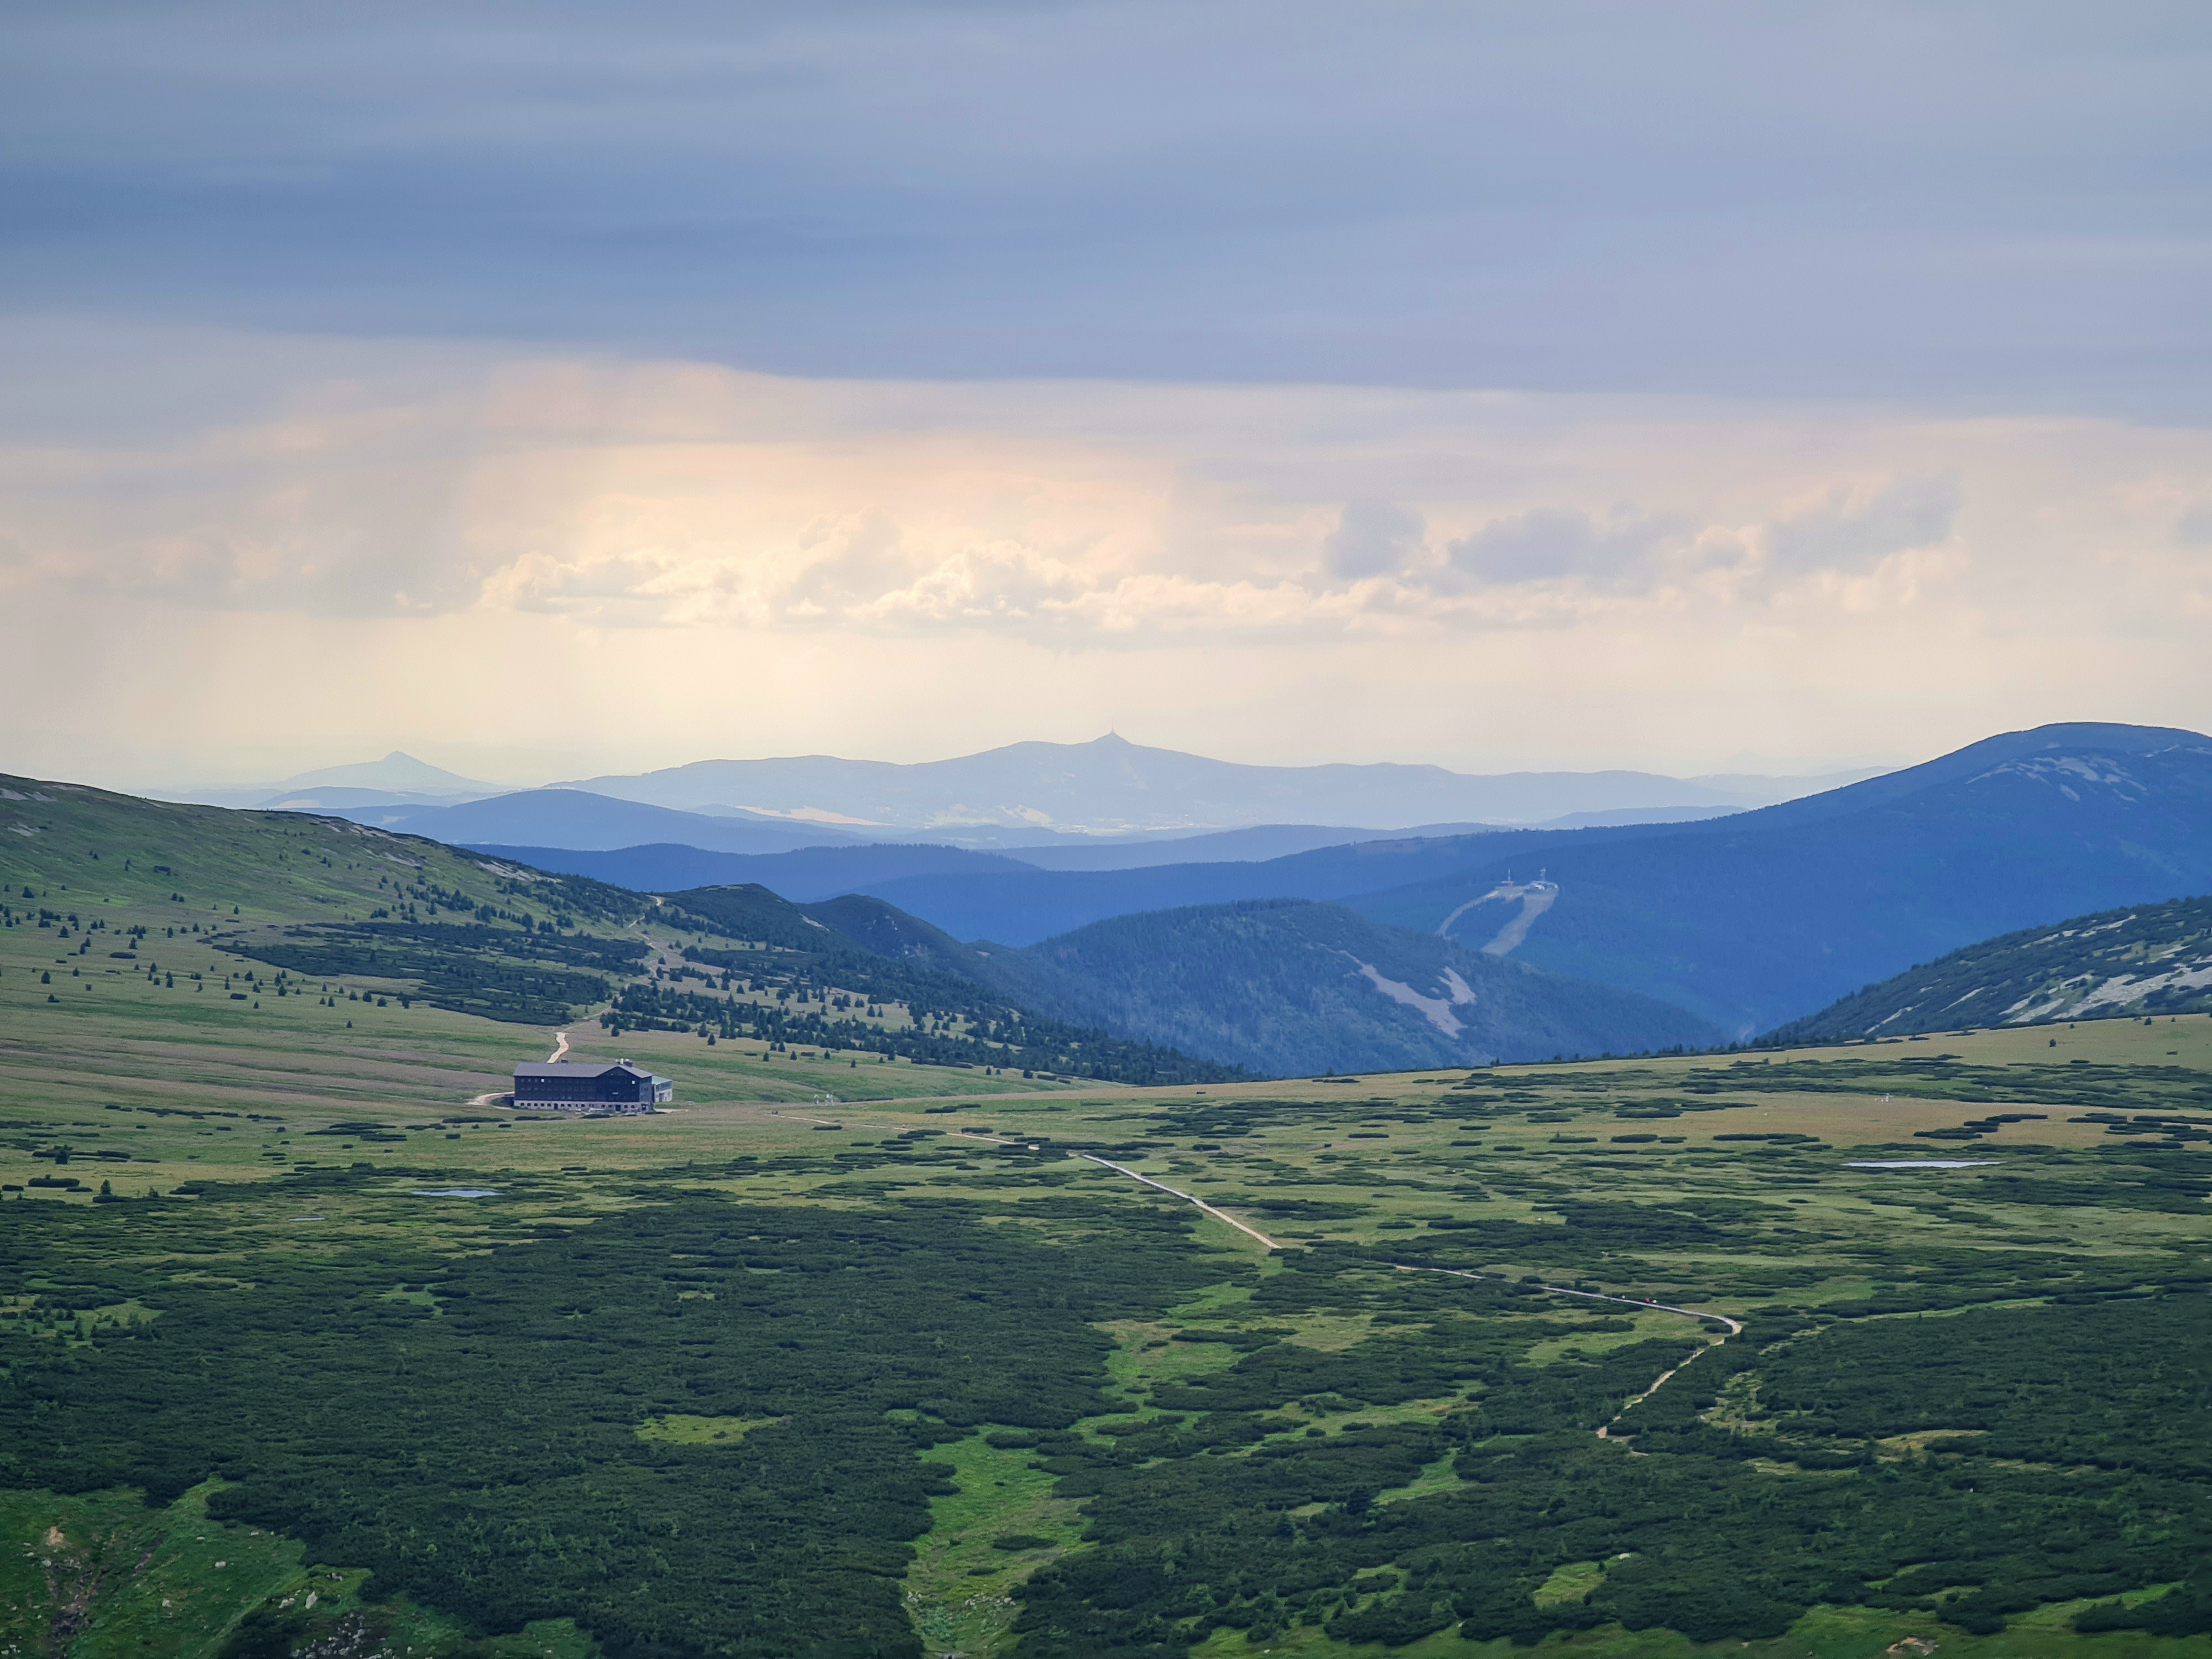
\includegraphics[width=0.75\textwidth]{sniezka.jpg}
    \caption{Widok ze Śnieżki (21.07.2023)} 
\end{figure}
\end{document}

